Based on your description, it seems like you want to create a TikZ LaTeX diagram that represents a hexagon with labeled parts. Here's an example code snippet that creates a similar hexagon with labeled sections:
```
\documentclass{article}
\usepackage{tikz}
\begin{document}
\begin{figure}[h]
\centering
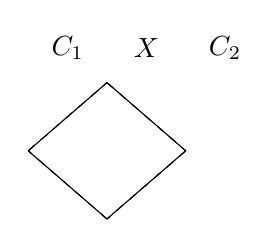
\begin{tikzpicture}
  % Draw the hexagon
  \draw (0,0) -- (1,0.866) -- (2,0) -- (1,-0.866) -- (0,0);
  
  % Label the sections of the hexagon
  \node at (0.5,1.3) {$C_1$};
  \node at (1.5,1.3) {$X$};
  \node at (2.5,1.3) {$C_2$};
  
  % Add lines to separate the sections
  \draw[dashed] (0,0) -- (1,0.866);
  \draw[dashed] (1,0.866) -- (2,0);
  \draw[dashed] (2,0) -- (1,-0.866);
  \draw[dashed] (1,-0.866) -- (0,0);
\end{tikzpicture}
\caption{Hexagon with labeled sections}
\label{fig:hexagon}
\end{figure}
\end{document}
```
This code will produce a hexagon with three sections labeled $C_1$, $X$, and $C_2$. The dashed lines separate the sections and make them easier to distinguish. You can customize the code further to fit your specific needs.